\chapter{Transformación de \emph{Bogoliubov} - 1/2}

	
\begin{tikzpicture}
	\fill [left color=red!50, right color=teal!50] (0,0) rectangle (6.5,.1);
	\fill [left color=teal!50, right color=blue!50] (6.5,0) rectangle (11.5,.1);
	\end{tikzpicture}



\vspace{10mm}
\begin{adjustwidth}{50pt}{50pt}
\begin{ejemplo}

Vamos a ver las transformaciones de Bogoluibov, que tienen importantísimas aplicaciones en superconducitividad, en superfluidos en en teoría cuántica de campos (TQC), sobre todo en el comportamiento de los campos en las cercanías del horizonte de sucesos de los agujeros negros.

En vez de trabajar con las coordenadas $q,p$, lo haremos con las $a,a^*$

\end{ejemplo}
\end{adjustwidth}
\vspace{5mm}
\section{Transformación de \emph{Bogoliubov}}

\begin{definition}

Recordemos lo obtenido en el capítulo anterior para el oscilador armónico \textcolor{gris}{(usaremos la notación de primas para las $q$ y $p$ en vez de las tildes, por comodidad)}:

 $$q'=\sqrt{\frac{m\omega_0}{2\hbar}}\ q;\quad p'=\dfrac 1{\sqrt{2m\hbar \omega_0}}\ p \quad \to \quad H'=p'^2+q'^2=\dfrac{H}{\hbar \omega_0}$$
 
 $$a=q'+ip; \quad a^* =q'-ip \quad \Rightarrow \quad q'=\dfrac 1 2 (a+a^*);\quad p'=\dfrac i 2 (a-a^*)$$
\end{definition}

Empezamos con un ejemplo a modo de motivación y luego daremos la definición exacta de transformación de Bogoliubov.

!`Atención¡: aunque no se diga explícitamente, estamos trabajando con las coordenadas adimensionales $\ q',\ p'$.

\begin{example}

\vspace{2mm} Supongamos que tenemos un hamiltoniano de la forma, $\ H=\alpha \ a a^* + \beta \ (aa+a^*a^*)\ $	

\vspace{2mm} Nos piden que encontremos una transformación de $ \ a,a^* \ \to \ b,b^*\ , \ $ de modo que el nuevo hamiltoniano se escriba como $\ H=\lambda b b^*$

\vspace{2mm} Si esto es posible, se le llama \textbf{\emph{diagonalizar} el hamiltoniano} y nos sirve como ejemplo de transformación de Bogoliubov (que básicamente consiste en diagonalizar el hamiltoniano)

\vspace{2mm} La transformación que encontremos, $ \ a,a^* \ \to \ b,b^*\, , \  $ deberá ser \textbf{canónica}, para lo que o bién exigimos que $|M|=1$ o que que las ecuaciones de Hamilton tengan la misma forma en ambas variables, $\ \dot a =\{a,H\} \ \to \ \dot b=\{b,H\} \ $
\end{example}

Probamos la siguiente transformación, $\quad \begin{cases} 
 \ b=ua+va^* \\ \ b^*=ua^*+va	
 \end{cases} \quad u,v\in \mathbb R$


Para que sea canónica ha de ocurrir que $|M|=1$, luego

$\displaystyle M=\mqty( \displaystyle \pdv {b}{a} & \displaystyle \pdv {b}{a^*} \\ \\ \displaystyle \pdv {b^*}{a} & \displaystyle \pdv {b^*}{a^*} )= \mqty(u&v\\v&u) \quad \to \quad |M|=\ \boxed{ \ \boldsymbol{u^2-v^2 = 1} \ }$

Una posibilidad es parametrizando en la forma: $\quad \begin{cases} \ u= \cosh \theta \\ \ v=\sinh \theta \end{cases}$
 

\begin{myalertblock}{Recordatorio: funciones hiperbólicas}
\begin{center}
\begin{multicols}{2}
$u^2+v^1=1 \to 	\begin{cases} \ u= \cos \theta \\ \ v=\sin \theta \end{cases} $

$(\cos^2 \theta + \sin^2 \theta=1,\ \ \forall \theta \in \mathbb R) $

$u^2+v^1=1 \to 	\begin{cases} \ u= \cosh \theta \\ \ v=\sinh \theta \end{cases} $

$(\cosh^2 \theta -\sinh^2 \theta=1,\ \ \forall \theta \in \mathbb R) $
\end{multicols}

\vspace{5mm}Algo más adelante necesitaremos las fórmulas del ángulo doble:

\begin{multicols}{2}

$\sin 2 \theta=2\sin \theta \cos \theta$

$\cos 2 \theta=\cos^2 \theta	 - \sin^2 \theta$

$\sinh 2 \theta=2 \sinh \theta \cosh \theta$

$\cosh 2 \theta= \cosh^2 \theta + \sinh^2 \theta$
\end{multicols}
\end{center}
\end{myalertblock}

\vspace{5mm} Nuestra transformación será $\quad \begin{cases}
\ b=\cosh \theta \ a \ + \ \sinh \theta \ a^* \\ \ b^*=\sinh \theta \ a^* \ + \ \cosh \theta \ a 	& \ \ \textcolor{gris}{\text{(conjugando  b)}}
 \end{cases}$

Para cada $\theta \in \mathbb R$ tendremos una transformación distinta. Elegiremos $\theta$  tal que cumpla con nuestro objetivo: conseguir expresar $H$ en la forma $\ H=\lambda \ bb^*$


Despejando $a,a^*$ en función de $b,b^*$, como se cumple que $\mqty(\cosh \theta & \sinh \theta \\ \sinh \theta & \cosh \theta ) ^{-1}=\mqty(\cosh \theta & -\sinh \theta \\ -\sinh \theta & \cosh \theta)$, relación que es sencilla de comprobar, es fácil obtener el cambio:
$\quad \begin{cases} \ a=\cosh \theta \ b - \sinh \theta \ b^* \\ \ a^*=-\sinh \theta \ b + \cosh \theta \ b^*  \end{cases}$ 

Calculemos los factores que aparecen en el hamiltoniano:

$\boldsymbol{ \triangleright } \quad aa^*=-csb^2+c^2bb^*+s^2bb^*-cs{b^*}^2=(\cosh^2 \theta+\sinh^2 \theta) \ bb^* \ - \ \cosh \theta \sinh \theta\  (b^2+{b^*}^2)$

--- $ \quad aa=c^2b^2+s^2{b^*}^2-2cs\ bb^*$ $\qquad$
--- $ \quad a^*a^*=(aa)^*=c{b^*}^2+s^2b^2-2sc\ bb^*$

$\boldsymbol{ \triangleright } \quad aa+a^*a^*=(c^2+s^2)b^2+(c^2+s^2){b^*}^2-4cs\ bb^* = (\cosh^2 \theta+\sinh^2 \theta) (b^2+{b^*}^2)-4\cosh \theta \sinh \theta \ bb^*$

Sustituyendo en el hamiltoniano,

\begin{small}
$H=\alpha \left[ (\cosh^2 \theta + \sinh^2 \theta) \ bb^* - \cosh \theta \sinh \theta \ (b^1+{b^*}^2 
\right] + \beta \left[
(\cosh^2 \theta + \sinh^2 \theta) \ (b^2+{b^*}^2) - 4\cosh \theta \sinh \theta \ bb^* 
\right]$
\end{small}

$H= \left[ \alpha(\cosh^2 \theta + \sinh^2 \theta)  -4\beta \cosh \theta \sinh \theta 
\right] \ bb^* +  \left[
- \alpha \cosh \theta \sinh \theta + \beta (\cosh^2 \theta + \sinh^2 \theta) 
\right] \ (b^2+{b^*}^2)$


Como nuestro objetivo es conseguir expresar $H$ en la forma $\ H=\lambda \ bb^*\, , \ $ entonces elegiremos

$\theta \ \ / \ \ -\alpha \cosh \theta \sinh \theta + \beta (\cosh^2 \theta + \sinh^2 \theta) \ = 0$

Usando las relaciones entre las funciones hiperbólicas comentadas anteriormente,

$ -\dfrac \alpha 2 \ \sinh 2\theta \ + \ \beta \ \cosh 2 \theta \ = \ 0$

Recapitulando, hemos de elegir el ángulo de modo

$$\subrayado{ \ 
\boldsymbol{
\theta \ \ / \ \ \text{si } \  -\dfrac \alpha 2 \ \sinh 2\theta \ + \ \beta \ \cosh 2 \theta \ = \ 0 \quad \Rightarrow \quad H=(\alpha \cosh 2 \theta - 2 \beta \sinh 2 \theta)\ bb^*
} \ }$$

Donde hemos utilizados las relaciones del ángulo doble para funciones hiperbólicas en la expresión del hamiltoniano obtenida anteriormente.


$ -\dfrac \alpha 2  \sinh 2\theta  +  \beta  \cosh 2 \theta =  0 \ \to \ \boldsymbol{\cosh 2\theta = \dfrac 1 \beta \dfrac \alpha 2 \sinh 2 \theta}$

Para resolver esta ecuación, nos ayudamos de la relación fundamental de las razones hiperbólicas:

$\begin{cases}
\ 	\cosh 2\theta = \dfrac 1 \beta \dfrac \alpha 2 \sinh 2 \theta \\ \ \cosh^2 2\theta - \sinh^2 2 \theta = 1 
\end{cases} \quad \left( \dfrac{\alpha}{2\beta} s \right)^2 - s^2=1 \to s^2 \left ( \left(  \dfrac{\alpha}{2\beta} s \right)^2 - 1 \right) =1 \to s^2=\dfrac 1 { \left(  \dfrac{\alpha}{2\beta} s \right)^2 - 1}$


$\sinh 2\theta=\dfrac 1 { \sqrt{\left(  \dfrac{\alpha}{2\beta} s \right)^2 - 1} }\ ;\qquad \cosh 2\theta= \dfrac {\alpha}{2\beta } \dfrac 1 { \sqrt{\left(  \dfrac{\alpha}{2\beta} s \right)^2 - 1} }$

Sustituyendo en el hamiltoniano:

$H=\left[ \alpha \ \dfrac {\alpha}{2\beta } \dfrac 1 { \sqrt{\left(  \dfrac{\alpha}{2\beta} s \right)^2 - 1} } - 2\beta \ \dfrac 1 { \sqrt{\left(  \dfrac{\alpha}{2\beta} s \right)^2 - 1} } \right] \ bb^* = \left( \alpha \dfrac {\alpha}{2\beta} - 2\beta \right) \ \dfrac{1}{\sqrt{\left(  \dfrac{\alpha}{2\beta} s \right)^2 - 1}}\ bb^*$

Como $\ \dfrac{\alpha^2}{2\beta}-2\beta=2\beta \left( \dfrac{\alpha^2}{4\beta^2}-1 \right) \quad \text{y} \quad \dfrac{\Box}{\sqrt{\Box}}=\sqrt{\Box}\, , \ $ tendremos


$H=2\beta \sqrt{\left(  \dfrac{\alpha}{2\beta} s \right)^2 - 1} \ bb^* = \sqrt{\alpha^2-4\beta^2}\ bb^*$


Realmente, este hamiltoniano es $H'$, que es igual a $\dfrac {H}{\hbar \omega_0}\, , \ $ por lo que

$\boldsymbol{ H=}\hbar \omega_0 \ \sqrt{\alpha^2-4\beta^2}\ bb^* \boldsymbol{= \hbar \ \Omega \ bb^*}$

se comporta como un oscilador de frecuencia $\ \quad \subrayado{ \ \boldsymbol{ \Omega=\sqrt{\alpha^2-4\beta^2}\ \omega_0} }$

\vspace{5mm} ?`Qué ha ocurrido físicamente? Es \emph{como si} hubiésemos cambiado de masa. Veamos que significa esto:

Como $a=q'+ip' \quad a^*=q`-ip' $, calculemos

$\triangleright \quad aa^*=q'^2+p'^2$

--- $aa=q'^2-p'^2+2iq'p' \ ; \qquad $ --- $a^*a^*=(aa)^*=q'^2-p'^2-2iq'p'\, \ $ por lo que

$\triangleright \quad aa+a^*a^*=2q'^2-2p'^2\ $ y entonces,

$H=(\alpha-2\beta)p'^2+(\alpha+2\beta)q'^2$

Con la relación de $q',p'$ con $q,p$ recordada en la introducción del tema,

$H=\hbar \omega_0\ \left[ (\alpha-2\beta) \dfrac{p^2}{2m \hbar \omega_0} + (\alpha+2\beta)\dfrac{m\omega_0^2}{2\hbar} q^2 \right] = (\alpha-2\beta) \dfrac {p^2}{2m} + (\alpha+2\beta)\dfrac{m\omega_0^2}{2}q^2$

$H=	\dfrac{p^2}{2m\dfrac{1}{\alpha-2\beta}} + \dfrac 1 2 (\alpha+2\beta) m\omega_0^2 q^2$

Reinterpretando una nueva masa $M$ como $M=m \dfrac 1{\alpha-2\beta} \ \to \ m=M(\alpha-2\beta)\, ,  \ $ podemos escribir

$H=\dfrac{p^2}{2M}+\dfrac 1 2 M ((\alpha^2-4\beta^2)\omega_0^2 q^2\ $ y teniendo en cuenta la nueva frecuencia $\Omega$,

$$\boxed{ \  \boldsymbol{ H \ = \ \dfrac{p^2}{2M} \ + \ \dfrac 1 2 M \Omega^2\ q^2} \ }$$


\underline{Interpretación}: $H=\dfrac{p^2}{2m}+ \dfrac 1 2 m\omega^2 q^2 \quad \wedge \quad  m\ \to \ M(\alpha-2\beta) \quad \Rightarrow \quad \omega_0 \ \to \ \Omega=\sqrt{\alpha^2-4\beta^2}\ \omega_0$

Con las variables $a, a^*$, el término $aa + a^* a^*$ es el responsable del \emph{``cambio de masas''}. Podemos interpretar que se trata de un muelle con una masa diferente.

\vspace{5mm}

\begin{ejemplo}
\begin{small}
	En superconductividad, $\beta <0 \to M=m(\alpha+2\beta), \ \text{si} \ \alpha=1 \to \Delta m=M-m=1+2|\beta|-1=2|\beta| \ \uparrow\, , \ $ la masa aumenta. Se llaman \emph{fermiones pesados} y son los responsables de la superconductividad. \end{small}
\end{ejemplo}

\vspace{10mm} Si calculamos $H^*=\alpha a^*a+ \beta(a^*a^*+aa)=H \ \Rightarrow \ H\in \mathbb R \quad $ \textcolor{gris}{(la energía es real, no compleja).} 


Trabajando con dos partículas podríamos tener 

$ H=\alpha_1 a_1a_1^* + \beta_1 (a_1a_1+a_1^*a_1^*) +\alpha_2 a_2a_2^* + \beta_2 (a_2a_2+a_2^*a_2^*) $

Pasando a coordenadas $q,p \ \to \ H=\dfrac 1{2M_1} p_1^2 + \dfrac{M_1}{2} \Omega_1 q_1^2 \ + \ \dfrac 1{2M_2} p_2^2 + \dfrac{M_2}{2} \Omega_2 q_2^2$

Se trata de dos osciladores armónicos de frecuencias $\Omega_1$ y $\Omega_2$ y masas \emph{efectivas} $M_1$ y $M_2$ \textbf{aislados}. que no interaccionan mutuamente.


\begin{figure}[H]
	\centering
	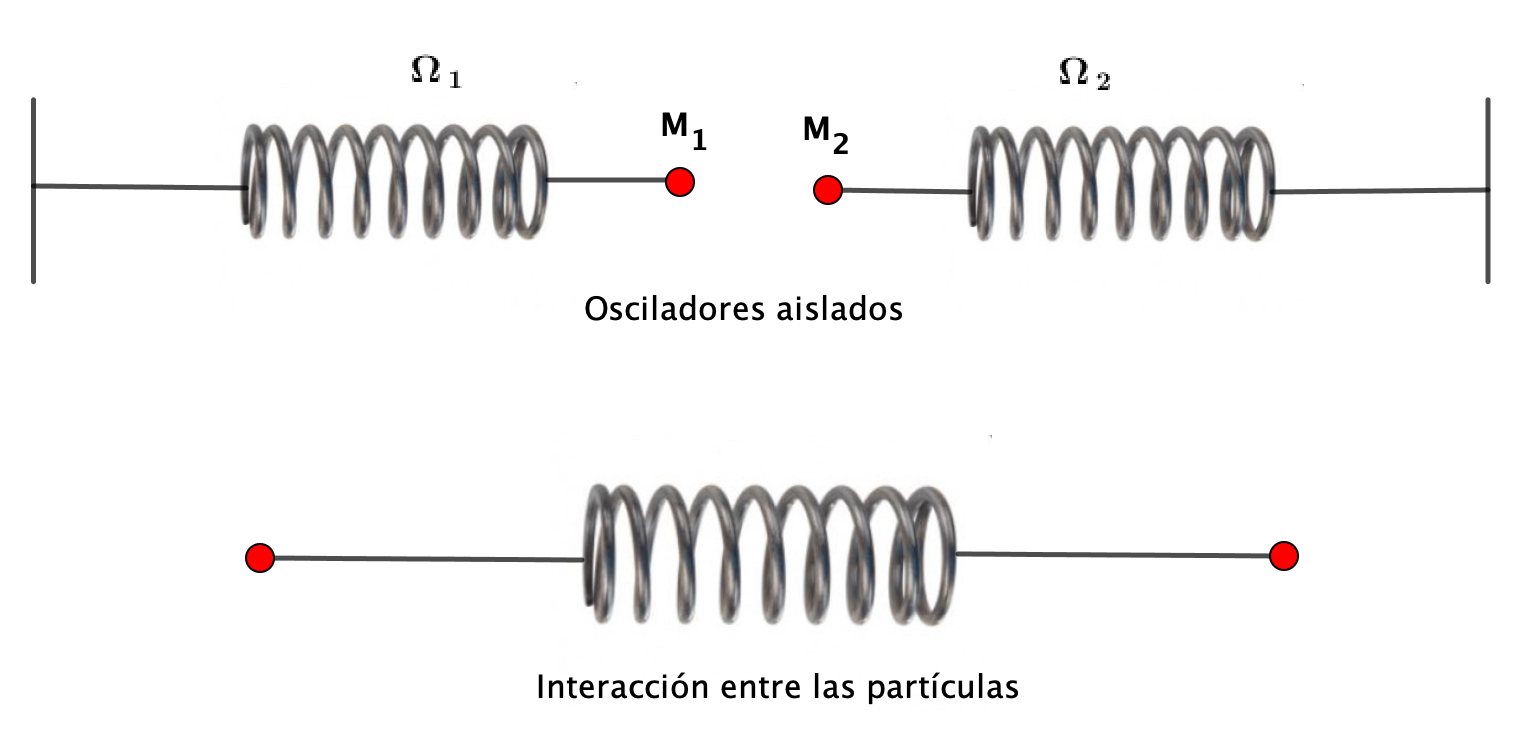
\includegraphics[width=.75\textwidth]{imagenes/img24-01.png}
\end{figure}

Para poder explicar más fenómenos, necesitamos  una interacción entre las partículas, por ejemplo,

$H=\dfrac{p_1^2+p_2^2}{2}+\dfrac{m\omega_0^2}{2} (q_1-q_2)^2=\dfrac{p_1^2+p_2^2}{2}+\dfrac{m\omega_0^2}{2} (q_1^2+q_2^2 \boldsymbol{-2q_1q_2} )=
\dfrac{p_1^2}{2} + \dfrac{m\omega_0^2}{2}q_1^2+\dfrac{p_2^2}{2} + \dfrac{m\omega_0^2}{2}q_2^2 \ - \ m\omega_0^2 \ q_1q_2$

El término del producto entre las $q_i$ hace que no se trate de osciladores aislados sino que exista una interacción entre ellos: $\ -2q_1q_2\  $ en términos de las $a,\ a^* $ es: $\quad$\textcolor{gris}{$\left(q'=\dfrac 1 2 (a+a^*)\right)$}

$-2q_1q_2=-2 \dfrac 1 4 (a_1+a_a^*)(a_2+a_2^*)=-\dfrac 1 2 (a_1a_2+a_1a_2^*+a_1^*a_2+a_1^*a_2^*)$, 

por lo que un $H$ genérico en que las dos partículas interaccionen entre sí podría ser:

$$\subrayado{ \ \boldsymbol{ H=\displaystyle \sum_{i=1}^2 \  [\alpha_1a_ia_i^* + \beta_i (a_ia_i + a_i^*a_i^*)] - \dfrac \lambda 2 [a_1a_2+a_1a_2^*+a_1^*a_2+a_1^*a_2^*] } \ }$$

Hamiltoniano adimensional en que puede haber un `cambio de masa', cuya primera parte corresponde a dos osciladores armónicos aislados y la segunda responde de la interacción entre ambos.

\vspace{5mm}
\begin{ejercicio}
En el próximo tema consideraremos el caso sencillo de que las dos partículas tengan la misma masa $m$ y estén unidas por un muelle de frecuencia $\omega_0$.

Como $\Omega=\sqrt{\alpha_1^2-4\beta_i^2}\ \omega_0$, si elegimos $\alpha_1=\ \alpha_2=1$ y $\beta_1=\beta_2=0 \ \to \ \Omega_1=\Omega_2=0$. Haciendo, por sencillez, $\lambda=1$,

 $H=a_1a_1^*+a_1a_2^*-\dfrac 1 2 [a_1a_2+a_1a_2^*+a_1^*a_2+a_1^*a_2^*]$
 
 Nuestro objetivo, en el siguiente capítulo, será encontrar $b_1, (b_1^*), b_2, (b_2^*)$ de modo que:
 
$\qquad  \begin{cases}
 \ b_1=u_{11}a_1+u_{12}a_2+v_{11}a_1^*+v_{12}a_2^* \\
 \ b_2=u_{21}a_1+u_{22}a_2+v_{21}a_1^*+v_{22}a_2^* \\  
 \ b_1^*=u_{11}a_1^*+u_{12}a_2^*+v_{11}a_1+v_{12}a_2 \\
 \ b_2^*=u_{21}a_1^*+u_{22}a_2^*+v_{21}a_1+v_{22}a_2  	
 \end{cases}\qquad \qquad $ Transformación de Bogoliubov.

Las $u_{ij},\ v_{ij}$ no pueden ser cualesquiera pues la transformación ha de ser \emph{canónica}.
\end{ejercicio}

\vspace{5mm}

\begin{ejemplo} En TQC se estudiará el conjunto de varios osciladores armónicos acoplados a los que, al aplicar una transformación de Bogoliubov, nos llevarán al concepto de \emph{campo cuántico}. \end{ejemplo}






